%% LyX 2.3.5.2 created this file.  For more info, see http://www.lyx.org/.
%% Do not edit unless you really know what you are doing.
\documentclass[english]{article}
\usepackage[T1]{fontenc}
\usepackage[latin9]{inputenc}
\usepackage{geometry}
\geometry{verbose,tmargin=1in,bmargin=0.5in,lmargin=1in,rmargin=1in}
\usepackage{graphicx}

\makeatletter

%%%%%%%%%%%%%%%%%%%%%%%%%%%%%% LyX specific LaTeX commands.
%% Because html converters don't know tabularnewline
\providecommand{\tabularnewline}{\\}

\makeatother

\usepackage{babel}
\begin{document}
Shengyi Liang

HPC

Prof. Peherstorfer

Homework 2

Here is my github address for homework: https://github.com/TonyLiang0518/Shengyi\_Liang\_HPC.git

\bigskip

1. 

test01:

First error is indexing out of range so changing i <= n to i < n can
fix the problem

Second error is mismatch between malloc and delete{[}{]}, changing
delete{[}{]} to free(x) works

\bigskip

test02:

The error is indexing uninitialized values at indices 2, 5-9 of x,
setting loop at line 81 to initialize all values of x fixes the problem

\bigskip

2.

I use Intel i9-9900K 3.6GHz 16 CPUs with 32GBs memory. 

Blocked version: 

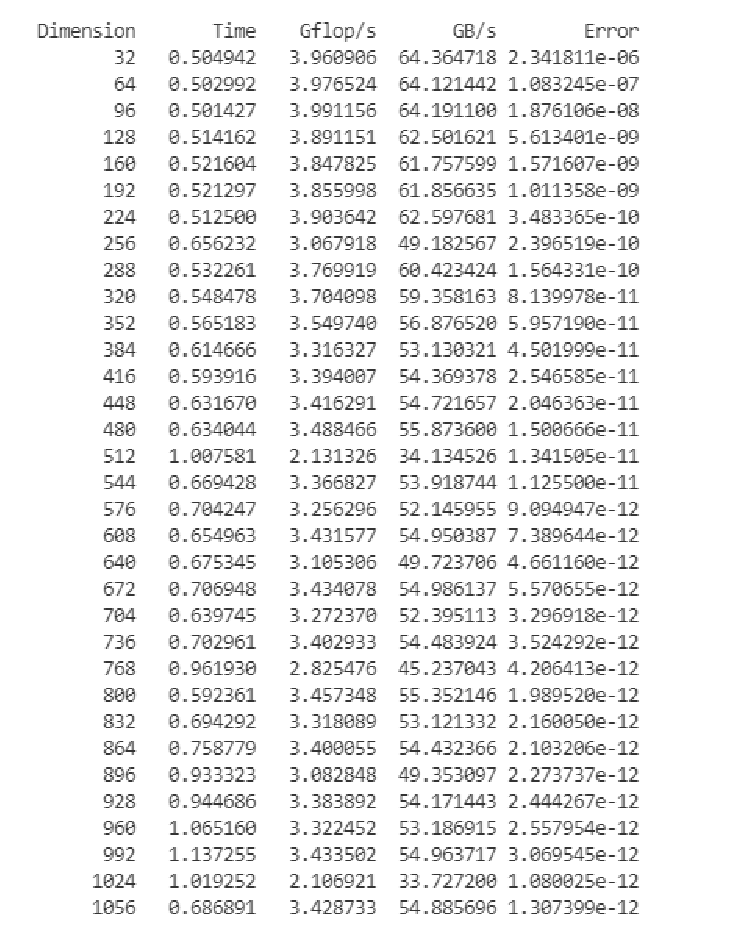
\includegraphics[scale=0.7]{hw2p2a}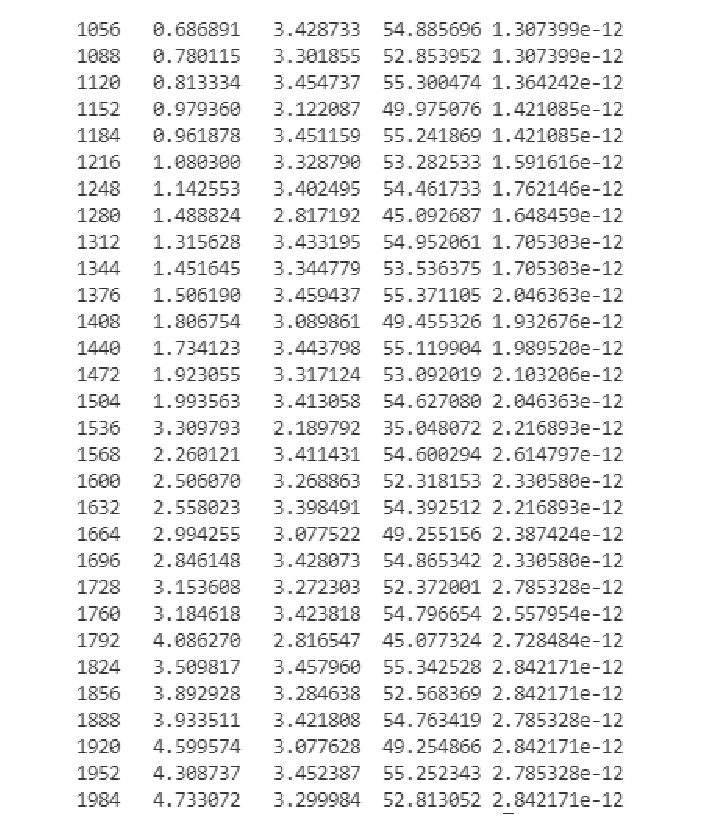
\includegraphics[scale=0.7]{hw2p2b}

\newpage{}

OpenMP optimized version: 

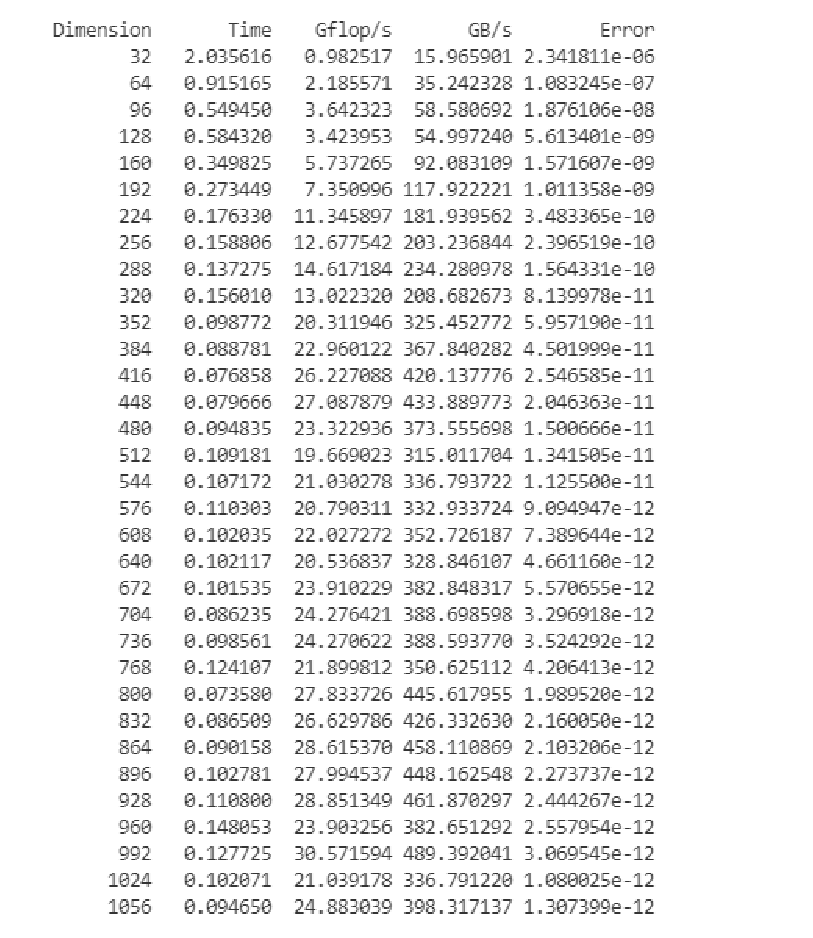
\includegraphics[scale=0.7]{hw2p2c}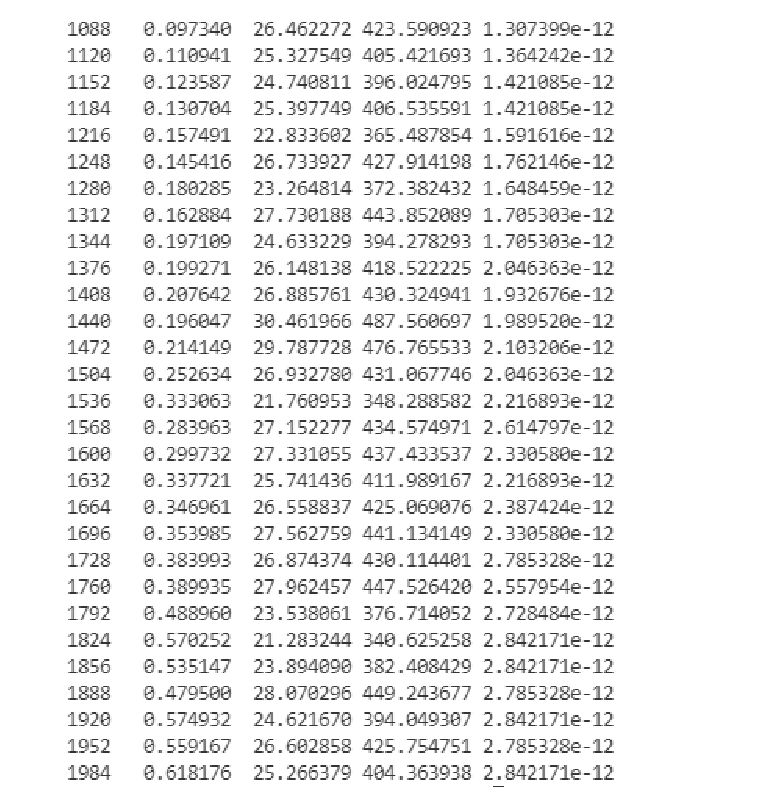
\includegraphics[scale=0.7]{hw2p2d}

\newpage{}

3.

omp\_bug2:

The error is the shared variables: $tid,i,total.$

By setting $private(tid)$ at line 18 and creating new parallel construct
at line 33 with $private(total,i)$, the issue is resolved. 

Another minor error is that the output does not always have ``Number
of threads = 16'' at the top, problem fixed by adding barrier at
line 27. 

\bigskip

omp\_bug3:

The error is at line 86, there is a barrier to wait for all threads
to execute and proceed but only two threads will eventually be able
to reach it. Problem fixed by commenting out the barrier

\bigskip

omp\_bug4:

The 2d array $a$ of size $1048*1048*sizeof(double)$ is too large
and there is no calculation involving double precision so problem
is fixed by initializing array $int$ $a[N][N]$

\bigskip

omp\_bug5:

There is a deadlock appears when two sections runs simultaneously.
After $locka$ is set in section 1, $lockb$ in section 2 may be set
as well; in this case, section 1 is unable to perform the operation
``adding $a${[}{]} to $b${[}{]}'' while section 2 is unable to
perform the operation ``adding $b${[}{]} to $a${[}{]}'' and a
deadlock appears. Moreover, it is also possible that when there is
only 1 thread, section 1 would lead to computation of uninitialized
values in $b$.

To fix this, I first set lock on both $a$ and $b$ at beginning of
section 1. After initialization ends in either section 1 or 2, unset
the lock on $a$ or $b$ so initialization will end for sure for both
$a$ and $b$. 

\bigskip

omp\_bug6:

1. $dotprod$ should be void, fixed by simply replacing $float$ by
$void$

2. $sum$ is initialized both in $main$ and $dotprod$ and not shared
properly, to fix this, I initialize it as global at line 15

\newpage{}

4.

I use Intel i9-9900K 3.6GHz 16 CPUs with 32GBs memory. 

\bigskip

Jacobi runtime:

\begin{tabular}{|c|c|c|c|}
\hline 
 & $N$=100 & $N$=200 & $N$=400\tabularnewline
\hline 
2 Threads & 0.210s & 3.283s & 51.034s\tabularnewline
\hline 
4 Threads & 0.136s & 1.921s & 30.785s\tabularnewline
\hline 
8 Threads & 0.122s & 1.310s & 19.708s\tabularnewline
\hline 
\end{tabular}

\bigskip

Gauss-Seidel runtime:

\begin{tabular}{|c|c|c|c|}
\hline 
 & $N$=100 & $N$=200 & $N$=400\tabularnewline
\hline 
2 Threads & 0.197s & 2.590s & 41.064s\tabularnewline
\hline 
4 Threads & 0.140s & 1.770s & 28.408s\tabularnewline
\hline 
8 Threads & 0.148s & 1.470s & 20.884s\tabularnewline
\hline 
\end{tabular}

\bigskip

As $N$ increases, the runtime increases as expected and each time
$N$ doubles, total runtime for same number of threads quadruples
since we compute in two dimensions. On the other hand, the iterations
needed quadruples as well which means the compute time for each iteration
is about the same for different $N$ due to OpenMP. 
\end{document}
